\documentclass[12pt]{report}
\usepackage[a4paper, left=0.5in, right=0.5in, top=0.5in, bottom=0.5in]{geometry}
\usepackage{xcolor}
\usepackage{amsmath}
\usepackage{amsthm}
\usepackage{amssymb}
\usepackage{amsfonts}
\usepackage{algpseudocode}
\usepackage{mathtools}
\usepackage{xcolor}
\usepackage{float}
\usepackage{framed}
\usepackage{listings}
\usepackage{graphicx}
\usepackage{subcaption}
\usepackage{tikz}
\usepackage{emoji}

\lstset{basicstyle=\ttfamily,
  commentstyle=\color{red},
  keywordstyle=\color{blue},
  %basicstyle=\footnotesize,
  frame=lines,
  numbers=left,
  stepnumber=1,
  showstringspaces=false,
  tabsize=1,
  breaklines=true,
  breakatwhitespace=false,
}
\usepackage{hyperref}
\hypersetup
{
    colorlinks=true,
    linkcolor=blue,
    filecolor=magenta,
    urlcolor=cyan,
    pdftitle={\Huge \textbf{CS218 Solutions NetworkFlow}},
    pdfpagemode=FullScreen,
}
\usepackage[utf8]{inputenc}
\usepackage{graphicx}
\usepackage{longtable}
\usepackage{multirow}
\usepackage{enumitem}
\setlength{\parindent}{0pt}

\begin{document}
\subsection*{\Large\bfseries Network Flow}
\begin{enumerate}[label=\textbf{\arabic*.}]

    \item
    \begin{itemize}
        \item Don't know, we know that vertex cover without the word `minimum' is in NP, but there's no clear way to show that a particular
        $k$ is minimum, how would you even give a proof that there is no vertex cover of size $k-1$ without brute force.
        \item Yes, this is in NP. We can actually just solve this problem in Polynomial time, as done in Q4 in Network Flow. So to 
        verify that the answer is $k$, we just solve it using our network flow algorithm and check if we also get $k$.
        \item Don't know, there's no clear way to prove that 2 programs are the same itself.
        \item Don't know, even though a proof could be just 2 inputs where the programs give different outputs, verifying this will take
        exponential time, either because the inputs could be exponentially large, or the program could take exponential time itself.
        \item Don't know. If we have some $n$ `for all's, we could have $2^n$ different choices of variables for which we have to verify 
        the formula as true, so a brute force proof will take exponential time. There is also no clear way to provide a shorter proof 
        in general, for any boolean formula.
    \end{itemize}

    \item We claim that a set is a vertex cover if and only if its complement (all vertices outside our set) is an independent set. If $S$
    is a vertex cover, for every edge $uv$, either $u \in S$ or $v \in S$. So there's no edge $uv$ where both $u \in S^c$ and $v \in S^c$. 
    But this is just saying $S^c$ is an independent set. Now for the converse, if $S$ is independent, there is no edge $uv$ such that 
    both $u \in S$ and $v \in S$. But this means for every edge, either $u \in S^c$ or $v \in S^c$, which is just saying $S^c$ is a vertex 
    cover. So if we want to check if we have an independent set of size $k$, we just need to check if we have a vertex cover of size $n-k$.
    This is because if there is an independent set of size $k$, the complement set will have size $n-k$ which is a vertex cover. And if we
    don't have an independent set of size $k$, we can't have a vertex cover of size $n-k$, else by our equivalence we can find an independent 
    set of size $n - (n-k) = k$.
    
    \item The idea is like this, we keep the elements of our sets as edges, since if we want to cover all edges it becomes equivalent to
    covering all elements of our sets. So our universe is going to be the set of all edges.
    And selecting a vertex should be equivalent to selecting some set right, so each set will just be set of all edges incident on our vertex.
    Now we claim that we have a vertex cover of size $k$ if and only if we have a set cover of size $k$. But this is obvious right, we just 
    select the corresponding sets we made for the vertex cover. Since every edge is incident with some vertex, every element is in some set.
    Similarly if we have a set cover of size $k$, we have a vertex cover of size $k$. Since any element is in some set, the corresponding edge 
    is incident with some vertex.

    \item For the load balancing problem, one machine is going to get some subset of $\{t_1, \dots, t_n\}$, and the other machine will get
    the rest of the elements. Let the subset of loads be $S$. The loads in each machine are $\sum_{i|t_i \in S} t_i$ and 
    $\sum_{i|t_i \notin S} t_i = \sum_i t_i - \sum_{i|t_i \in S} t_i$. Both of these should be at most $T$, from which we get the following 
    inequalities, $\sum_{i|t_i \in S} t_i \leq T$, and $\sum_{i|t_i \in S} t_i \geq \sum_i t_i - T$. The terms on the RHS of each inequality are 
    constants no matter what $S$ is. So we can see that this is now very similar to the knapsack problem. So our motivation will be like this,
    we are going to make sure $W_1, W_2$ add to sum of all the weights (by adding a new weight $w'$), 
    so that we can reduce to load balancing. So let's do that.

    Let $w'$ be such that $\sum_i w_i + w' = W_1 + W_2$ i.e. $w' = W_1 + W_2 - \sum_i w_i$, we are adding this new weight to our list of weights,
    and are now going to do load balancing with $T = W_2$. If we have a solution for this, choose the set of loads which don't have $w'$, and 
    call this set $S$. We know that $\sum_{i|w_i \in S} w_i \leq T = W_2$, now let's write the inequality for the other set.

    \begin{align*}
        \sum_{i|w_i \notin S} w_i + w' &\leq T = W_2 \\
        \sum_i w_i - \sum_{i|w_i \in S} w_i + W_1 + W_2 - \sum_i w_i &\leq W_2 \\
        W_1 &\leq \sum_{i|w_i \in S} 
    \end{align*}

    So this subset satisfies the knapsack constraints. The converse is also easy to show i.e. if a subset satisfies the knapsack constraints, it's
    going to satisfy the load balancing constraints, by just going backwards. We already know the subset without $w'$ has a sum $\leq W_2$, now for the 
    subset with $w'$.

    \begin{align*}
        \sum_{i| w_i \in S} w_i &\geq W_1 \\
        \sum_{i| w_i \in S} w_i + \sum_{i| w_i \notin S} w_i + W_2 &\geq W_1 + W_2 + \sum_{i| w_i \notin S} w_i \\
        \sum_i w_i + W_2 &\geq W_1 + W_2 + \sum_{i| w_i \notin S} w_i \\
        W_2 &\geq W_1 + W_2 - \sum_i w_i + \sum_{i| w_i \notin S} = w' + \sum_{i| w_i \notin S} w_i
    \end{align*}

    \item Each variable in our formula $\phi$ can be a variable in our linear equations. If $x_1, \dots, x_n$ are the variables, we put the 
    constraints $0 \leq x_i \leq 1$ to ensure each variable is 0 or 1. Now how do we write clauses? Take the clause $x_1 \lor \lnot x_2 \lor x_4$.
    To satisfy this clause we need at least one of $x_1, \lnot x_2, x_4$ to be 1. This can be actually represented as $x_1 + (1 - x_2) + x_4 \geq 1$.
    So we'll have $2n + k$ different linear inequalities ($n$ for all $x_i \geq 0$, $n$ for all $x_i \leq 1$, $k$ for each clause).

    \item We'd like to create a graph where there's a cycle corresponding to all of the $2^n$ possible assignments to variables $x_1, \dots, x_n$.
    How we do this is as follows, we make a path for each $x_i$, which can be traversed forwards and backwards. If moving from left to right, it's
    like assuming $x_i$ is 1, and right to left denotes assigning $x_i$ as 0. We will have connecting edges to move from 1 variable to the next,
    and one source and sink vertex. The length of each path is going to be twice the number of clauses (we'll see why we need this length later,
    just assume we choose some random length for now). Assume we have 4 variables, $x_1$ to $x_4$.

    \begin{figure}[H]
        \centering
        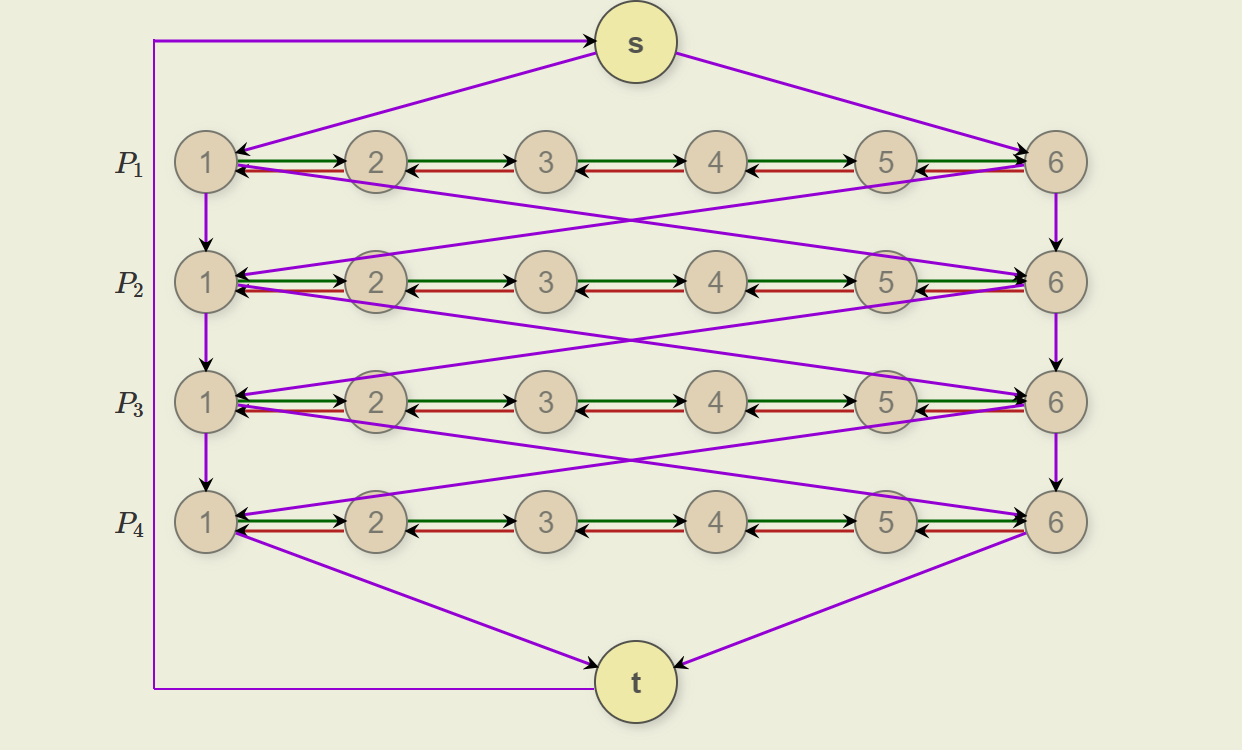
\includegraphics[width=0.5\textwidth]{Hamiltonian1.png}  
    \end{figure}

    In the above graph, there will be $2^4$ Hamiltonian cycles, because for each row, we can either go left to right, or right to left. We can't 
    backtrack on any path because each vertex has to be visited exactly once, and each can correspond to some assignment.

    Now we have to bring in the clauses. We add a node for each clause, and need to make sure it is visited only if the clause is satisfied.
    Let's say our first clause $C_1$ is $x_1 \lor x_2 \lor \lnot x_3$. So whenever $x_1$ is true i.e we move left to right in row 1, we should 
    be able to visit $C_1$. So what we do is add an edge from 1 in row1 to $C_1$, and an edge from $C_1$ to 2 in row 1. So instead of going straight
    from 1 to 2, we can divert to $C_1$ and come back. Since we have $\lnot x_3$, we need to be able to visit $C_1$ while going from right to left.
    So we add an edge from 2 in row 3 to $C_1$, and an edge from $C_1$ to 1 in row 3. We're only going to use the first and second nodes in each row 
    for $C_1$, these are allocated for $C_1$. Similarly third and fourth nodes are for $C_2$, fifth and sixth nodes are for $C_3$. Why are we keeping
    different nodes for each clause? This is because the same assignment can make multiple clauses true, maybe even all clauses so we want to have
    the option of allowing an assignment to visit any number of clauses while moving along the row. Below is how the graph will look after filling
    everything for $C_1$, and also we have the full graph if $C_2$ is $\lnot x_2 \lor x_3 \lor x_4$, and $C_3$ is $x_1 \lor \lnot x_2 \lor x_4$.

    \begin{figure}[H]
        \centering
        \begin{subfigure}[b]{0.45\textwidth}
            \centering
            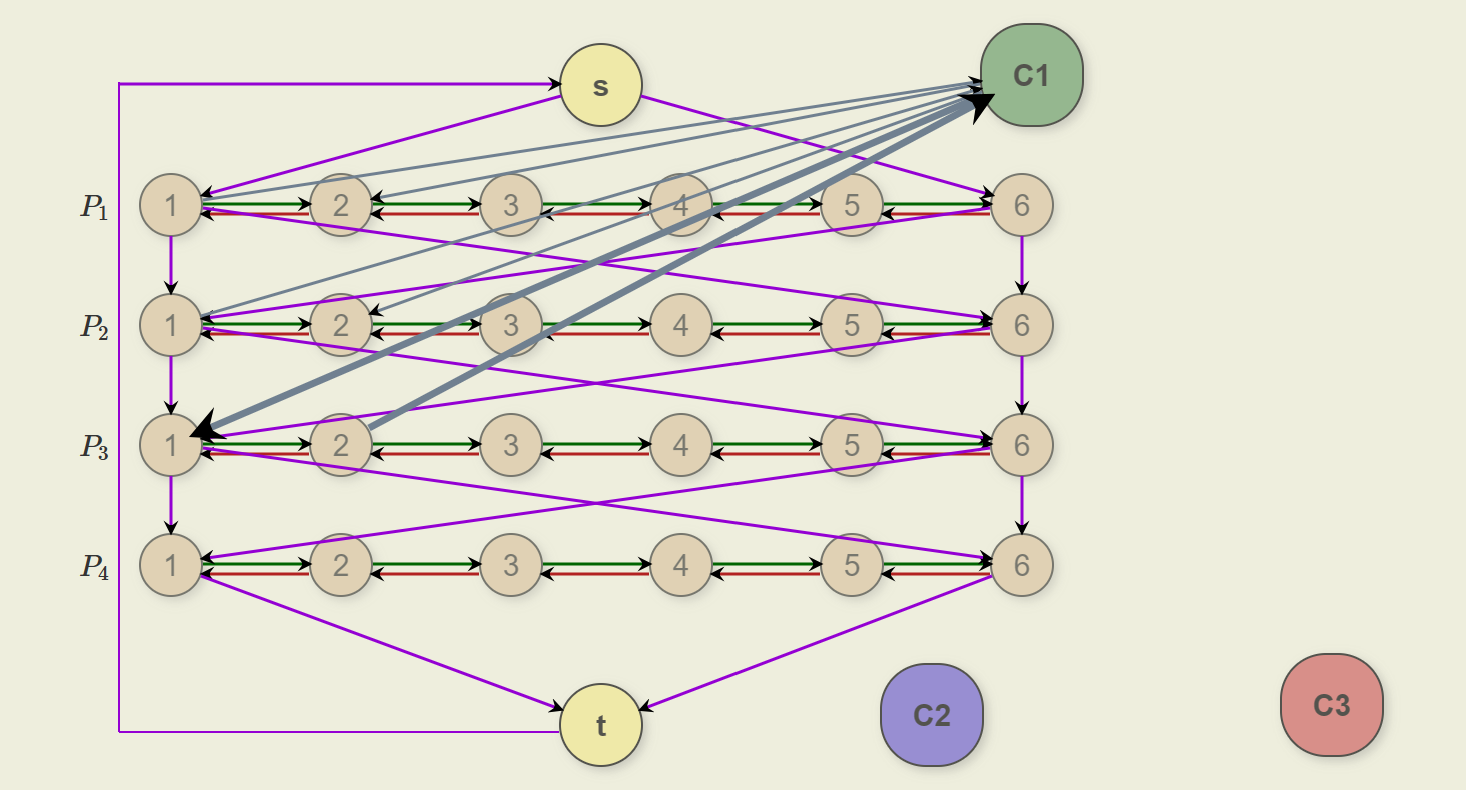
\includegraphics[width=\textwidth]{C1Hamiltonian.png}
            \caption*{After Clause 1}
        \end{subfigure}
        \hfill
        \begin{subfigure}[b]{0.45\textwidth}
            \centering
            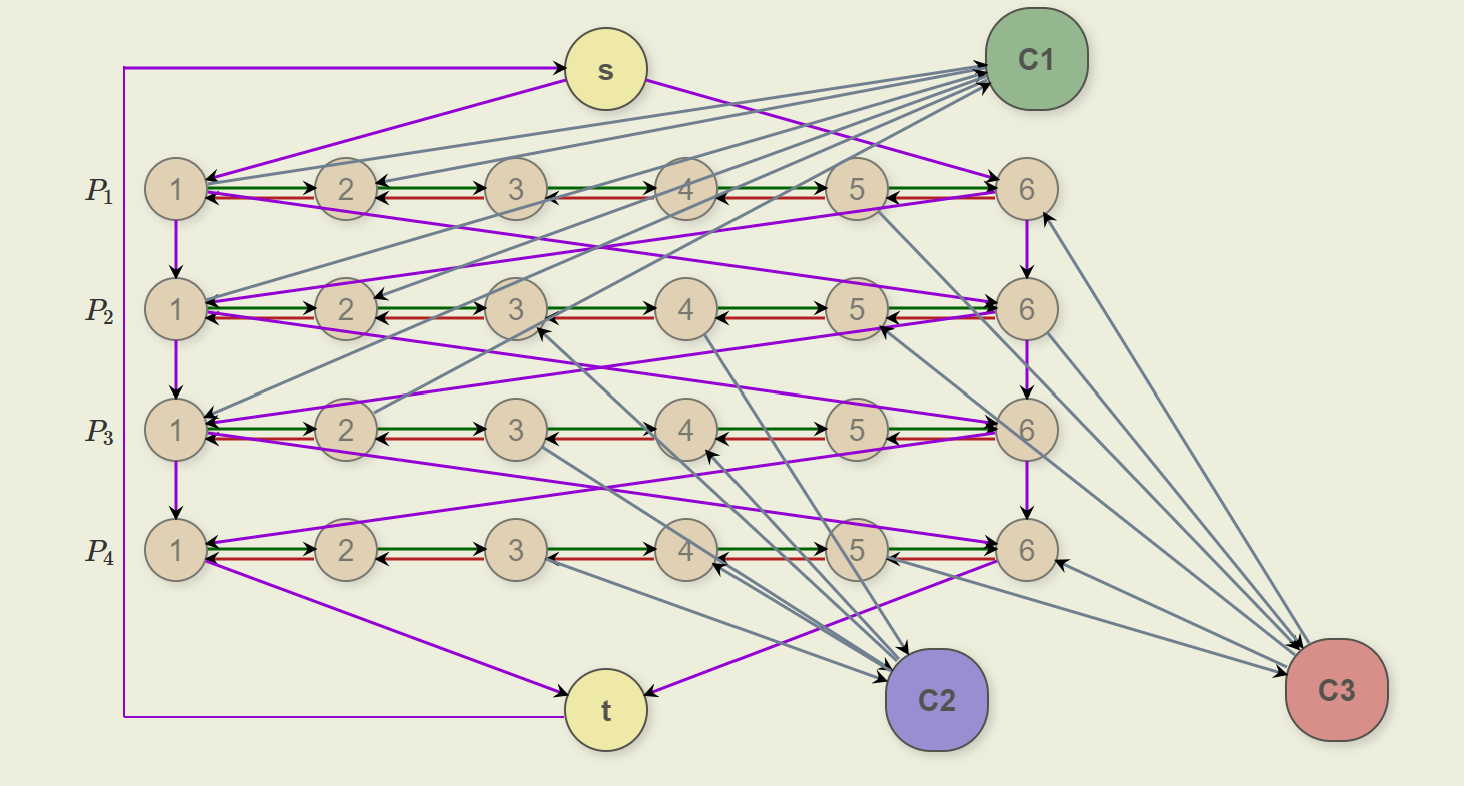
\includegraphics[width=\textwidth]{FinalHamiltonian.png}
            \caption*{Final Graph}
        \end{subfigure}
    \end{figure}

    Now if we find a Hamiltonian cycle in the graph, we can easily find out the assignment which works. Just see in which direction we move in 
    each row, and correspondingly assign each variable. This will satisfy the assignment as the Hamiltonian cycle visits every clause, meaning 
    at least one variable assignment is there to make every clause true. Similarly, if we have a satisfying assignment we'll definitely have a
    Hamiltonian cycle. We can find out in which direction to move through each row from the assignment. Since the assignment is satisfying, there 
    will be at least 1 variable assignment making each clause true, and whatever that is, we can take a detour there and visit that clause. Since
    we allocated different sections for each variable connecting to each clause, this is feasible.


\end{enumerate}
\end{document}